\problem{CT reconstruction}
The filted back projection is applied with the following steps: \\
1. Compute the $1-$D Fourier transform of each projection. \\
2. Multiply each $1-$D Fourier transform by the ramp filter which has been multiplied by a Hamming window. \\
3. Then obtain the inverse $1-$D Fourier transform of each resulting filtered projection. \\
4. For each projection, we replicate it, rotate it, and sum them together to obtain the reconstructed result. \\
The Hamming window is defined as:
$$w(n) = 0.54 - 0.46 \cos\left(\frac{2\pi n}{N-1}\right), \quad n = 0, 1, \ldots, N-1$$
where $N$ is the number of samples in the projection. \\
The normalized reconstructed image in shown in Figure \ref{fig:p1}.

\begin{figure}[htbp]
    \centering
	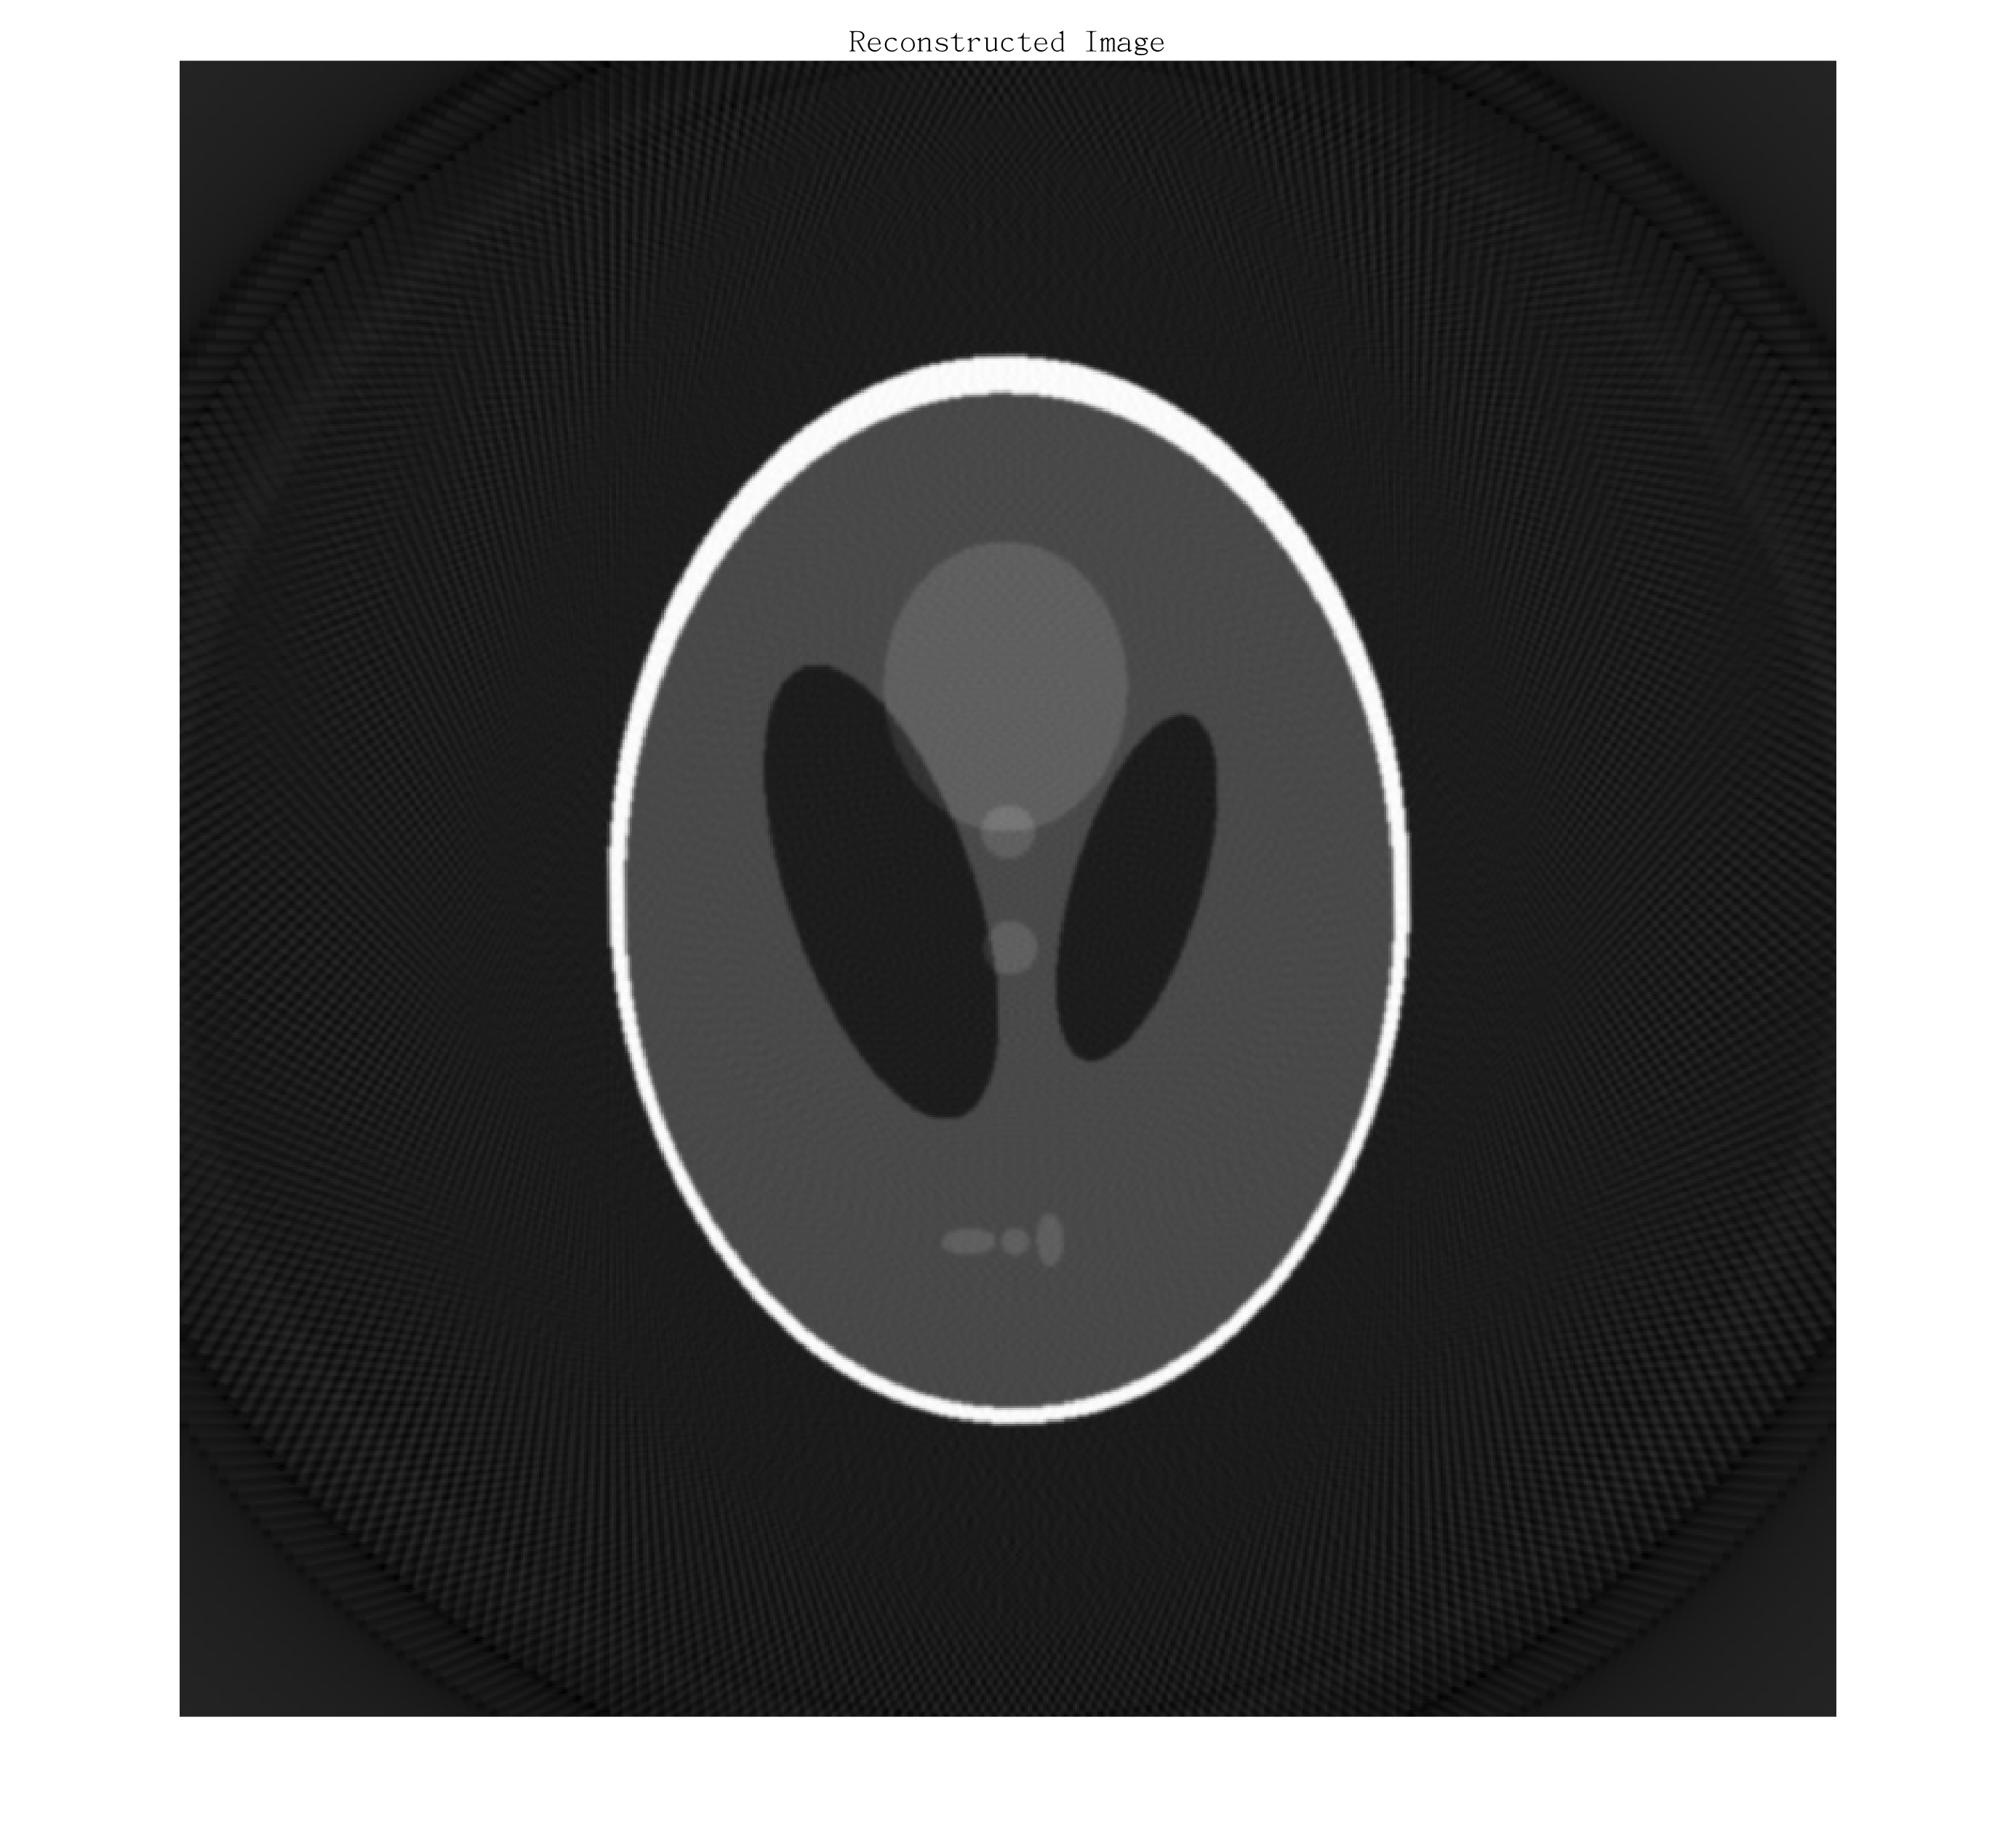
\includegraphics[width=0.9\textwidth]{../images/p1/p1.png}
    \caption{Reconstructed result of CT.}
    \label{fig:p1}
\end{figure}

\newpage